
\subsubsection{\pagerank}


First, we study the condition under which $\phi$-fairness and group-adpated $\phi$-fairness can be achieved by the FairGD and CrossGD algorithms. We run the FairGD on the Blogs and Twitter with a uniform restart vector. We vary the target PageRank scores of the two groups and record the fairness loss $L$ and the relative change to the transition matrix $\delta$ with FairGD and baselines. 
% The results are shown in Table~\ref{tab:blogs} and Table~\ref{tab:twitter}.

\haoyun{We can add a null baseline that does not change the transition matrix, to show the initial fairness loss.}

\haoyun{The losses are often very close to zero. We might use a logarithmic scale.}

\haoyun{The results for varying target PageRank ratios can be shown in figures. 
Each figure shows a metric (fairness loss or relative change) with respect to the target PageRank ratio.}

% For Blogs dataset, we find that the fairness loss with FairGD algorithm 
% is approximately zero when the target PageRank ratios range from 0.3 to 0.7 
% for the first group, indicating that the $\phi$-fairness in PageRank scores is achieved. 
% In these cases, FairGD outperforms LFBRU and LFBRN in terms of 
% the relative change to the transition matrix. 
% Especially when the target PageRank ratios are close to 0.5, 
% the relative change to the transition matrix with FairGD 
% is significantly smaller than that with LFBRU and LFBRN.

% For Twitter dataset, the FairGD algorithm achieves $\phi$-fairness in PageRank scores 
% when the target PageRank ratios range from 0.4 to 0.5 for the first group. 
% Again, FairGD outperforms LFBRU and LFBRN in terms of 
% the relative change to the transition matrix.

The Blogs and Twitter datasets contain two groups.
We vary the target \pagerank scores of the two groups
from 0.2 to 0.8 and from 0.8 to 0.2, respectively.
% As shown in Table~\ref{tab:blogs} and Table~\ref{tab:twitter},
when the target \pagerank scores are close to the initial \pagerank scores,
FairGD has a significantly smaller relative change to the transition matrix
than LFBRU and LFBRN, while having an almost zero fairness loss.
In these cases, FairGD also outperforms FairWalk and CrossWalk in terms of the Fairness loss.

The other datasets contain more than two groups. 
We set the target PageRank scores $\phi$ proportional to the number of vertices in each group, 
indicating the demographic parity. 
% From Table~\ref{tab:multi}, we observe that the FairGD algorithm achieves
$\phi$-fairness in PageRank scores for all datasets,
with the fairness loss close to zero.
In terms of the relative change to the transition matrix,
FairGD outperforms all baseline methods in all datasets.
In terms of the fairness loss, FairGD also outperforms FairWalk and CrossWalk.

% We notice the relationship between the performance of FairGD and the modularity of the network.

\begin{figure*}[htbp] % Use figure* for spanning across two columns
    \centering
    \begin{subfigure}[b]{0.45\textwidth}
        \centering
        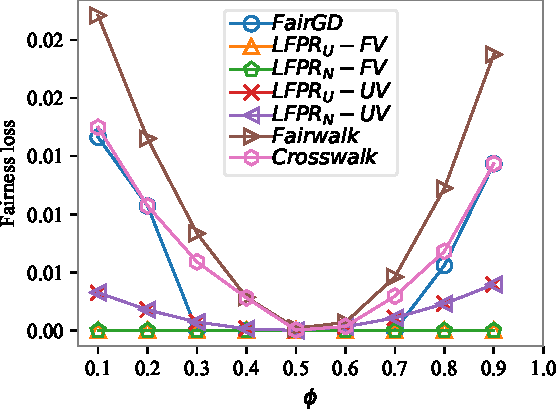
\includegraphics[width=\textwidth]{fig/blogs_fairness Loss.pdf} % Avoid spaces in filename
        \caption{Fairness loss with $\phi$ in $[0.1, \cdots, 0.9]$}
        \label{fig:unconstraint_blog_loss}
    \end{subfigure}
    \hfill
    \begin{subfigure}[b]{0.45\textwidth}
        \centering
        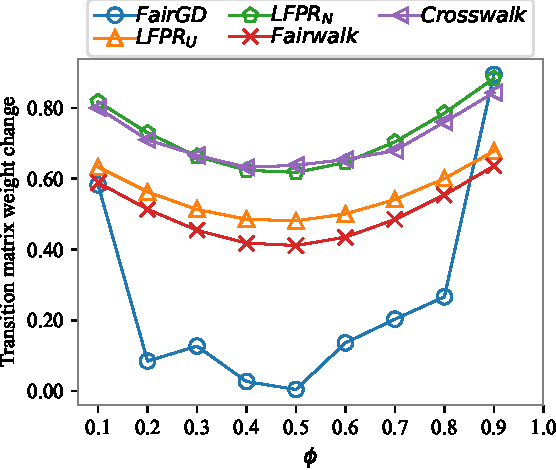
\includegraphics[width=\textwidth]{fig/blogs_Weight Change.pdf} % Avoid spaces in filename
        \caption{Transition matrix weight change with $\phi$ in $[0.1, \cdots, 0.9]$}
        \label{fig:unconstraint_blog_weight_change}
    \end{subfigure}
    \caption{Fairness loss and transition matrix weight change on the Blog dataset.}
    \label{fig:unconstraint_phi_plot_blog}
\end{figure*}
\todo{



\iffalse
\begin{figure*}[htbp] % Use figure* for spanning across two columns
    \centering
    \begin{subfigure}[b]{0.45\textwidth}
        \centering
        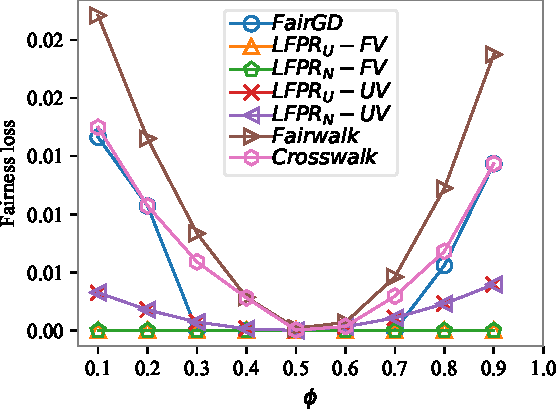
\includegraphics[width=\textwidth]{fig/blogs_fairness Loss.pdf} % Avoid spaces in filename
        \caption{Fairness loss with $\phi$ in $[0.1, \cdots, 0.9]$}
        \label{fig:basic_blog_fair}
    \end{subfigure}
    \hfill
    \begin{subfigure}[b]{0.45\textwidth}
        \centering
        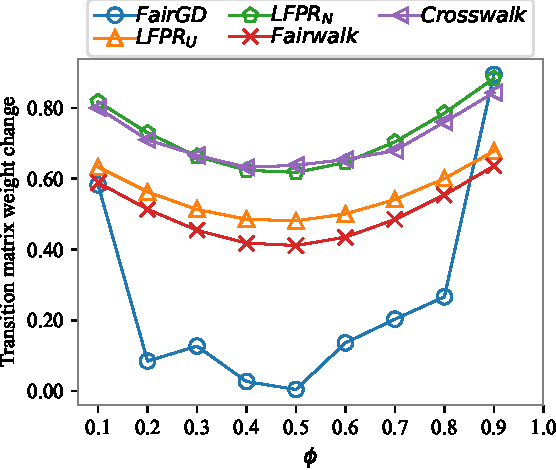
\includegraphics[width=\textwidth]{fig/blogs_Weight Change.pdf} % Avoid spaces in filename
        \caption{Transition matrix weight change with $\phi$ in $[0.1, \cdots, 0.9]$}
        \label{fig:basic_blog_weight}
    \end{subfigure}
    \caption{Fairness loss and transition matrix weight change on the Blog dataset with $\delta = 0.05$.}
    \label{fig:basic_blog}
\end{figure*}
\fi
\begin{figure*}[htbp] % Use figure* for spanning across two columns
    \centering
    \begin{subfigure}[b]{0.45\textwidth}
        \centering
        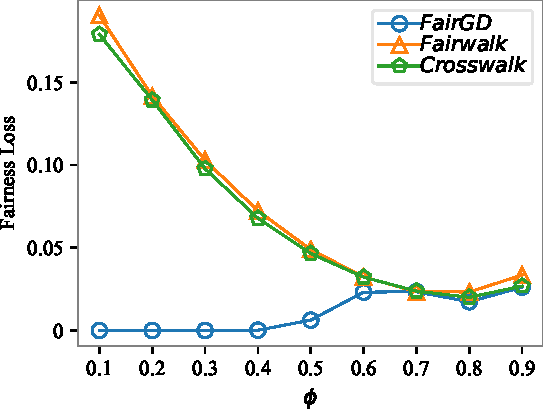
\includegraphics[width=\textwidth]{fig/books_fairness Loss.pdf} % Avoid spaces in filename
        \caption{Fairness loss with $\phi$ in $[0.1, \cdots, 0.9]$}
        \label{fig:basic_book_fair}
    \end{subfigure}
    \hfill
    \begin{subfigure}[b]{0.45\textwidth}
        \centering
        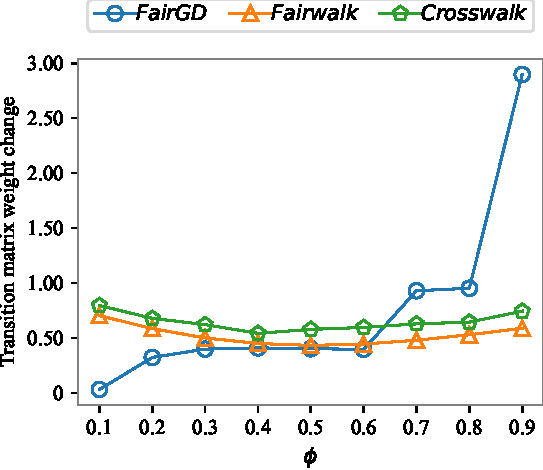
\includegraphics[width=\textwidth]{fig/books_Weight Change.pdf} % Avoid spaces in filename
        \caption{Transition matrix weight change with $\phi$ in $[0.1, \cdots, 0.9]$}
        \label{fig:basic_book_weight}
    \end{subfigure}
    \caption{Fairness loss and transition matrix weight change on the books dataset.}
    \label{fig:basic_book}
\end{figure*}


\begin{figure*}[htbp] % Use figure* for spanning across two columns
    \centering
    \begin{subfigure}[b]{0.45\textwidth}
        \centering
        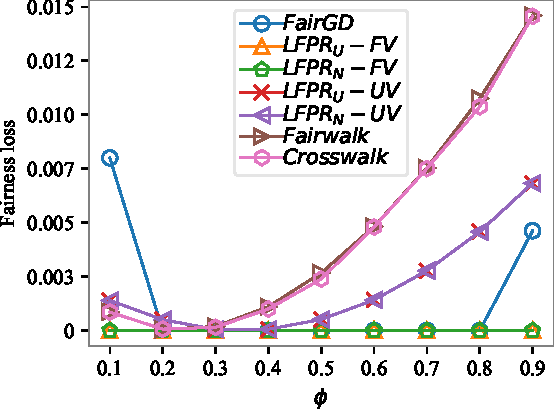
\includegraphics[width=\textwidth]{fig/mind_fairness Loss.pdf} % Avoid spaces in filename
        \caption{Fairness loss with $\phi$ in $[0.1, \cdots, 0.9]$}
        \label{fig:basic_mind_fair}
    \end{subfigure}
    \hfill
    \begin{subfigure}[b]{0.45\textwidth}
        \centering
        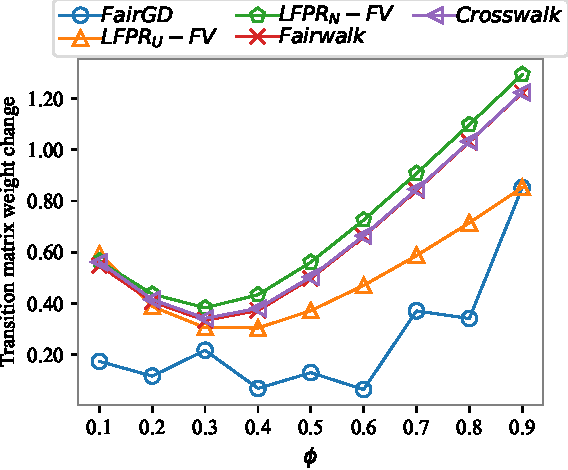
\includegraphics[width=\textwidth]{fig/mind_Weight Change.pdf} % Avoid spaces in filename
        \caption{Transition matrix weight change with $\phi$ in $[0.1, \cdots, 0.9]$}
        \label{fig:basic_mind_weight}
    \end{subfigure}
    \caption{Fairness loss and transition matrix weight change on the mind dataset.}
    \label{fig:basic_mind}
\end{figure*}

\begin{table*}[h!]
    \centering
    \begin{tabular}{c|ccccccccc}
        \hline
        $\phi$ & $\delta = 0.05$ & $\delta = 0.1$ & $\delta = 0.15$ & $\delta = 0.2$ & $\delta = 0.25$ & $\delta = 0.3$ & Fairwalk & Crosswalk \\
        \hline
        0.1 & 103.7 & 100.8 & 98.97 & 97.20 & 95.50 & 93.94 & 133.4 & 123.9 \\
        0.2 & 48.58 & 47.30 & 46.05 & 44.85 & 43.69 & 42.63 & 100.5 & 94.66 \\
        0.3 & 14.50 & 13.80 & 13.13 & 12.49 & 11.88 & 11.35 & 88.72 & 85.43 \\
        0.4 & 0.417 & 0.306 & 0.213 & 0.139 & 0.082 & 0.043 & 98.09 & 96.46 \\
        0.5 & 5.431 & 5.008 & 4.600 & 4.209 & 3.831 & 5.862 & 128.6 & 128.2 \\
        0.6 & 30.17 & 29.16 & 28.16 & 27.18 & 26.22 & 31.13 & 180.2 & 180.2 \\
        0.7 & 74.91 & 73.31 & 71.73 & 70.15 & 68.59 & 76.36 & 253.0 & 252.6 \\
        0.8 & 139.7 & 137.5 & 135.3 & 133.1 & 131.0 & 141.5 & 346.8 & 345.3 \\
        0.9 & 224.4 & 221.6 & 218.9 & 216.1 & 213.3 & 226.7 & 461.8 & 458.0 \\
        \hline
    \end{tabular}
    \caption{Fairness loss for the Twitter dataset, with rows corresponding to $\phi$ and columns to FairGD algorithm with$\delta \in [0.05, 0.3]$, fairwalk, and crosswalk. All values are multiplied by $10^{-3}$.}
    \label{tab:constraint_twitter_loss}
\end{table*}

\begin{table*}[h!]
    \centering
    \begin{tabular}{c|ccccccccccc}
        \hline
        $\phi$ & $\delta = 0.05$ & $\delta = 0.1$ & $\delta = 0.15$ & $\delta = 0.2$ & $\delta = 0.25$ & $\delta = 0.3$ & $LFPR_U$ & $LFPR_N$ & Fairwalk & Crosswalk \\
        \hline
        0.1 & 22.98 & 46.23 & 76.79 & 93.08 & 141.99 & 193.89 & 609.7 & 640.7 & 231.2 & 575.5 \\
        0.2 & 25.55 & 51.55 & 68.11 & 104.9 & 120.5 & 157.1 & 554.8 & 582.2 & 198.6 & 564.2 \\
        0.3 & 26.50 & 53.81 & 70.03 & 108.9 & 123.97 & 124.8 & 515.7 & 538.8 & 169.9 & 542.7 \\
        0.4 & 23.32 & 45.57 & 71.76 & 84.61 & 111.3 & 134.0 & 495.5 & 514.5 & 147.5 & 522.8 \\
        0.5 & 22.21 & 39.18 & 61.93 & 88.09 & 105.8 & 0.119 & 495.8 & 511.9 & 134.5 & 540.4 \\
        0.6 & 22.98 & 40.36 & 63.78 & 80.95 & 109.6 & 0.275 & 516.8 & 531.4 & 133.8 & 533.5 \\
        0.7 & 21.82 & 43.68 & 69.06 & 87.36 & 105.5 & 0.430 & 555.9 & 570.7 & 145.5 & 549.5 \\
        0.8 & 23.16 & 40.70 & 64.40 & 81.82 & 111.1 & 0.585 & 610.1 & 626.0 & 167.0 & 567.9 \\
        0.9 & 21.15 & 42.34 & 66.98 & 85.15 & 102.7 & 0.738 & 676.1 & 693.7 & 195.1 & 590.1 \\
        \hline
    \end{tabular}
    \caption{Transition matrix weight change for the Twitter dataset, with rows corresponding to $\phi$ and columns to FairGD algorithm with $\delta \in [0.05, 0.3]$, $LFPR_U$,$LFPR_N$, Fairwalk, and Crosswalk. All values are multiplied by $10^{-3}$.}
    \label{tab:constraint_twitter_wdiff}
\end{table*}

